\chapter{Permanent Memory and Buffer Management}
The first problem to be solved in implementing a DBMS is to \textbf{provide a level of abstraction} of the permanent memory that makes the \textit{other modules of the system} \textbf{independent} of its characteristics and of those of the storage system. All of this is achieved with the \textbf{Permanent Memory Manager} and \textbf{Buffer Manager}.

\section{Permanent Memory}
The memory managed by a DBMS is usually organized in a two-level hierarchy: the \textbf{temporary memory} (or main) and the \textbf{permanent memory} (or secondary).
\begin{itemize}
    \item \textbf{Main/Temporary memory}
    \begin{itemize}
        \item Electronic
        \item Fast access to data
        \item Small capacity
        \item Volatile
        \item Expensive
    \end{itemize}
    \item \textbf{Permanent memory with magnetic disks}
    \begin{itemize}
        \item Slow access to data
        \item Large capacity
        \item Non volatile
        \item Cheap
    \end{itemize}
    \item \textbf{Permanent memory with NAND flash memory}
    \begin{itemize}
        \item Relatively fast access to data 
        \item Medium capacity
        \item Non volatile (Persistent)
        \item Relatively expensive
    \end{itemize}
\end{itemize}
The flash memory, with the decrease in the cost and the increase in their capacity, is destined to establish itself for personal computers as an alternative to magnetic disks. However they poses new challenges to the implementation of DBMSs, due to timing characteristics.
\begin{figure}[!h]
        \centering
        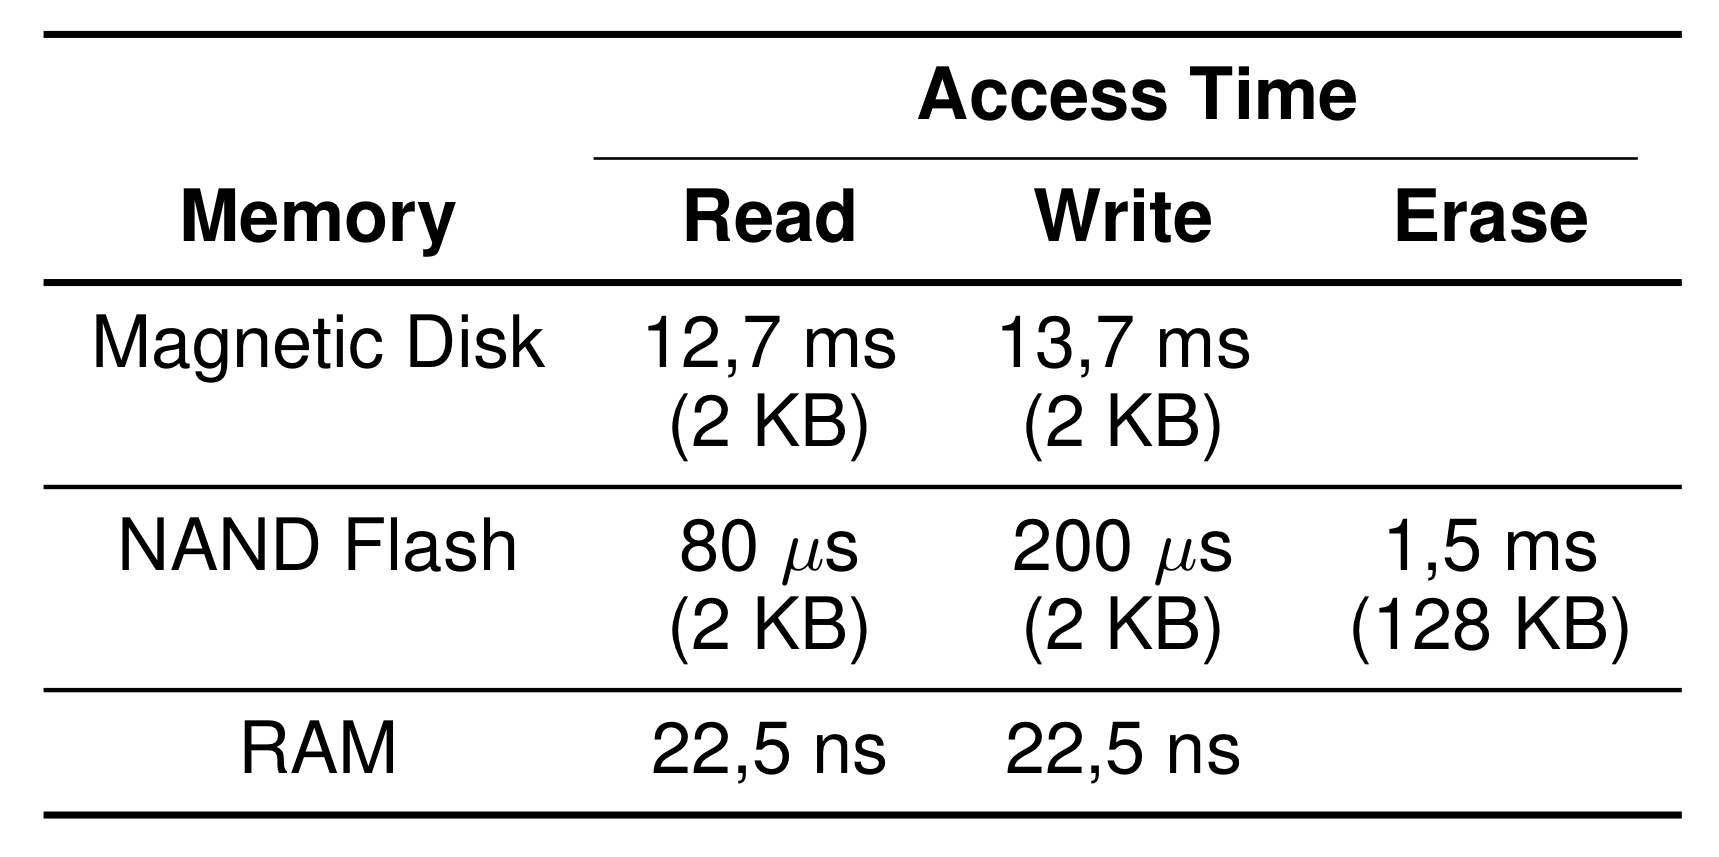
\includegraphics[width=0.5\linewidth]{images/DBMS_Internals/memory_types.jpeg}
        \caption{Characteristics of the three types of memory}
    \end{figure}
\begin{itemize}
    \item The reading and writing of data are faster than those of magnetic disks, but the rewriting of data is problematic because the data must be deleted first
    \item The erasing of data concerns several blocks called \textbf{memory unit} which should all be read to be deleted
    \item This type of memory becomes unreliable after 100 000 cycles of cancellations/rewrites
\end{itemize}

\subsection{Parentheses on Magnetic Disk}

\begin{itemize}
    \item A magnetic disk is composed of a pile of \(p\) \textbf{platters} with concentric rings called \textbf{tracks} used to store data
    \item A \textbf{track} is the part of the disk that can be used without moving the read head and it is divided in \textit{sectors} of the same size, which are the smallest unit of transfer allowed by the hardware and cannot be changed
    \item A \textbf{track} is logically divided in \textit{blocks} of fixed with a multiple of sector size
    \item The disk driver has an array of \textbf{disk heads}, one per recorded surface. Each head is fixed on a movable arm that displaces the head horizontally on the entire surface of a disk
    \item A \textbf{cylinder} is the set of tracks of the surfaces of the disks that can be used without moving the heads
\end{itemize}
The time to read or write a block, called the \textbf{access time}, has the following components:
\begin{itemize}
    \item The \textbf{seek time \(t_s\):} time needed to position the disk heads over the cylinder containing the desired block
    \item The \textbf{rotational latency \(t_r\):} the time spent waiting for the desired block to appear under the read/write head
    \item The \textbf{transfer time \(t_b\):} the time to read or write the data in the block once the head is positioned
\end{itemize}
The transfer time fora single block in the temporary memory is then \((t_s + t_r + t_b)\), while the transfer time for k contiguous blocks is \((t_s + t_r + k \times t_b)\).

Moreover since \textit{seek time} + \textit{latency} is much greater than \textit{transfer time}, it is important: 
\begin{itemize}
    \item To transfer greater blocks rather than small ones
    \item Makes consecutive reads on consecutive blocks on the  same cylinder
\end{itemize}

\section{Permanent Memory Manager}
\begin{itemize}
    \item The Permanent Memory Manager takes care of the \textit{allocation} and \textit{de-allocation} of pages within a database, and performs \textit{reads} and \textit{writes} of pages to and from the disk
    \item It provides an \textbf{abstraction of the permanent memory} in terms of a set of databases each made of a set of files with page-sized blocks of bytes, called \textbf{physical pages}
    \begin{itemize}
        \item The physical pages of a file are numbered consecutively starting from zero
        \item Can grow dynamically, limited to the permanent memory available space
        \item When it is transferred to the main memory it is called a \textbf{page}
    \end{itemize}
\end{itemize}

\newpage
\section{Buffer Manager}
\begin{itemize}
    \item Its role is to make pages from the permanent memory available to transactions in the main memory
    \item It is responsible to to allow transactions to get the pages they need, while minimizing disk access operations, by implementing a page replacement strategy
\end{itemize}
The performance of operations on a database depends on the number of pages transferred to temporary memory. The cost of some operations may be reduced by using a buffer capable of containing many pages.


The buffer manager uses the following structures to carry out its tasks:
\begin{figure}[!h]
        \centering
        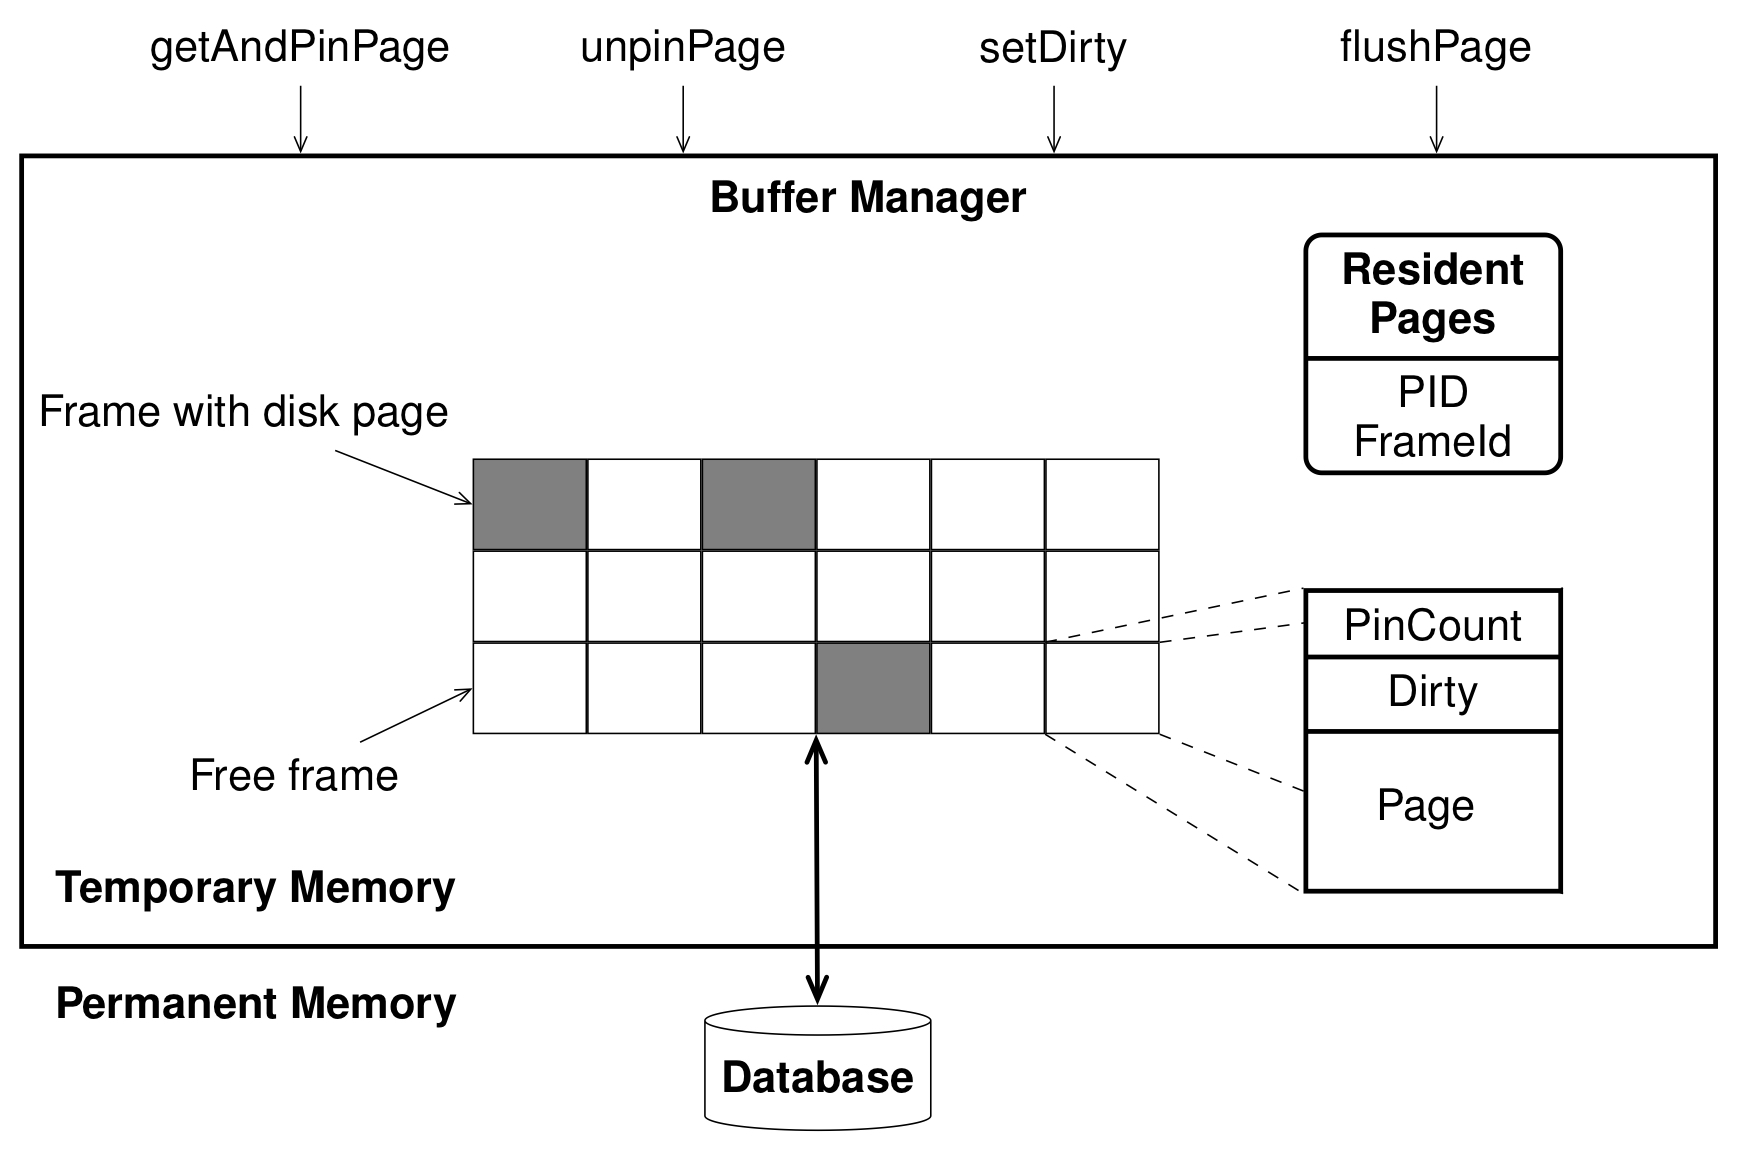
\includegraphics[width=0.7\linewidth]{images/DBMS_Internals/bufgfer_managment.jpeg}
        \caption{The Buffer Manager}
    \end{figure}
    
\begin{itemize}
    \item The \textbf{buffer pool:}
    \begin{itemize}
        \item It is an array of frames each one containing a copy of a permanent memory page
        \item It has a fixed size, so when there are no free frames, in order to copy a new page from the permanent memory an appropriate algorithm is used in order to free a frame
        \item To manage it in a frame are also stored two variables:
        \begin{itemize}
            \item \textit{pin count:} initially \textit{false} and it stores the number of times that the page currently in the frame has been requested but not released
            \item \textit{dirty bit:} initially \(0\) and it indicate whether the page has been modified
        \end{itemize}
    \end{itemize}
    \item A hash \textbf{resident pages} tables, called \textbf{directory:}  used to know if a permanent memory page, with a given page identifier PID, is in the buffer pool, and which frame contains it
\end{itemize}
    
The buffer manager provides the following primitives to use the pages in the buffer pool:\begin{itemize}
    \item \textit{getAndPinPage(P):} iff a frame contains the requested page, it increments the pin count of that frame and returns the page identifier to the requester. And if the requested page is not in the buffer pool, it is brought in as follows:
    \begin{enumerate}
        \item A free frame is chosen according to the buffer management’s replacement policy, most often \textit{Least Recently Used (LRU)}. If the frame chosen for replacement is dirty, the buffer manager flush it. If there are no free frames an exception is raised
        \item The requested page is read into the frame chosen for replacement and \textit{pinned}
        \item The resident pages table is updated, to delete the entry for the old page and insert an entry for the new page
    \end{enumerate}
    \item \textit{setDirty(P):} if the requestor modifies a page, it asks the buffer manager to set the dirty bit of the frame
    \item \textit{unpinPage(P):}w hen the requestor of a page releases the page no longer needed, it asks the buffer manager to unpin it
    \item \textit{flushPage(P)} the requestor of a page asks the buffer manager to write the page to the permanent memory if it is dirty
\end{itemize}